%%%%%%   TIPO DE DOCUMENTO: Artículo   %%%%%%
\documentclass[letterpaper,11pt,twoside]{article}

\usepackage[spanish]{babel}
\usepackage{graphicx}
\usepackage[utf8]{inputenc}
\usepackage{hyperref}
\usepackage{xspace}
\usepackage{listings}
\usepackage{amsmath, amssymb, amscd, amsthm}
\usepackage{makeidx}
\usepackage{algpseudocode}
\usepackage{algorithm}
\usepackage{float}
\usepackage{caption}

% Ajustes de márgenes
\setlength{\textheight}{23cm}
\setlength{\textwidth}{15cm}
\setlength{\oddsidemargin}{0.5cm}
\setlength{\evensidemargin}{0.5cm}
\setlength{\topmargin}{-1cm}

\captionsetup[figure]{position=below, skip=5pt}

\begin{document}
	
	\begin{center}
		{\bf \Large Compiladores} \\
		\today \\
		\vspace{0.5cm}
		\textbf{Martínez Buenrostro Jorge Rafael} \\
		\textit{correo: cbi2203040824@izt.uam.mx} \\
		Universidad Autónoma Metropolitana \\
		Unidad Iztapalapa, México
	\end{center}
	
	\section*{Introducción}
	El presente reporte describe la implementación de cuatro Autómatas Finitos Deterministas (AFD) diseñados para reconocer lenguajes regulares específicos. La implementación se realizó en lenguaje C, utilizando estructuras de datos para representar la lógica de estados y transiciones.
		
	\section*{Análisis de Autómatas}
	
	\subsection*{1. Expresión Regular $a^*ba^*$}
	Este autómata acepta cadenas que contienen exactamente una letra 'b', precedida y seguida por cualquier cantidad de letras 'a'.
	
	\textbf{Definición Formal:}
	$M_1 = \{Q, \Sigma, \delta, q_0, F\}$, donde:
	\begin{itemize}
		\item $Q = \{q_0, q_1, q_2\}$
		\item $\Sigma = \{a, b\}$
		\item $s = q_0$
		\item $F = \{q_1\}$
	\end{itemize}
	
	\textbf{Tabla de Transiciones:}
	\begin{table}[H]
		\centering
		\begin{tabular}{|c|c|c|}
			\hline
			Estado & \textbf{a} & \textbf{b} \\ \hline
			$q_0$  & $q_0$      & $q_1$      \\ \hline
			$q_1$  & $q_1$      & $q_2$		 \\ \hline
			$q_2$  & $q_2$      & $q_2$      \\ \hline
		\end{tabular}
	\end{table}
	
	\begin{figure}[H]
		\centering
		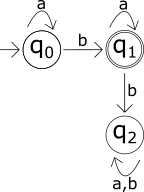
\includegraphics{img/automata1.png}
		\caption{Diagrama del autómata para $a^*ba^*$}
	\end{figure}
	
	\subsection*{2. Expresión Regular $a^*bba^*$}
	Acepta cadenas que contienen la subcadena exacta 'bb', con cualquier cantidad de 'a' alrededor, pero sin permitir más 'b's.
	
	\textbf{Definición Formal:}
	$M_2 = \{Q, \Sigma, \delta, q_0, F\}$, donde:
	\begin{itemize}
		\item $Q = \{q_0, q_1, q_2, q_3\}$
		\item $\Sigma = \{a, b\}$
		\item $s = q_0$
		\item $F = \{q_2\}$
	\end{itemize}
	
	\textbf{Tabla de Transiciones:}
	\begin{table}[H]
		\centering
		\begin{tabular}{|c|c|c|}
			\hline
			Estado & \textbf{a} & \textbf{b} \\ \hline
			$q_0$  & $q_0$      & $q_1$      \\ \hline
			$q_1$  & $q_3$      & $q_2$      \\ \hline
			$q_2$  & $q_2$      & $q_3$      \\ \hline
			$q_3$  & $q_3$      & $q_3$      \\ \hline
		\end{tabular}
	\end{table}
	
	\begin{figure}[H]
		\centering
		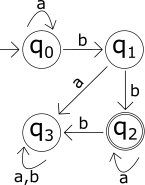
\includegraphics{img/automata2.png}
		\caption{Diagrama del autómata para $a^*bba^*$}
	\end{figure}
	
	\subsection*{3. Expresión Regular $a^*b^*$}
	Reconoce cadenas que tienen cero o más 'a' seguidas de cero o más 'b'. Una vez que aparece una 'b', no puede volver a aparecer una 'a'.
	
	\textbf{Definición Formal:}
	$M_3 = \{Q, \Sigma, \delta, q_0, F\}$, donde:
	\begin{itemize}
		\item $Q = \{q_0, q_1, q_2\}$
		\item $\Sigma = \{a, b\}$
		\item $s = q_0$
		\item $F = \{q_0, q_1\}$
	\end{itemize}
	
	\cleardoublepage
	
	\textbf{Tabla de Transiciones:}
	\begin{table}[H]
		\centering
		\begin{tabular}{|c|c|c|}
			\hline
			Estado & \textbf{a} & \textbf{b} \\ \hline
			$q_0$  & $q_0$      & $q_1$      \\ \hline
			$q_1$  & $q_2$      & $q_1$      \\ \hline
			$q_2$  & $q_2$      & $q_2$      \\ \hline
		\end{tabular}
	\end{table}
	
	\begin{figure}[H]
		\centering
		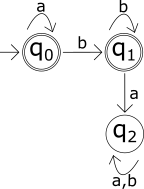
\includegraphics{img/automata3.png}
		\caption{Diagrama del autómata para $a^*b^*$}
	\end{figure}
	
	\subsection*{4. Expresión Regular $a^*ba^*ba^*$}
	Este autómata acepta cadenas que contienen exactamente dos letras 'b'.
	
	\textbf{Definición Formal:}
	$M_4 = \{Q, \Sigma, \delta, q_0, F\}$, donde:
	\begin{itemize}
		\item $Q = \{q_0, q_1, q_2, q_3\}$
		\item $\Sigma = \{a, b\}$
		\item $s = q_0$
		\item $F = \{q_2\}$
	\end{itemize}
	
	\textbf{Tabla de Transiciones:}
	\begin{table}[H]
		\centering
		\begin{tabular}{|c|c|c|}
			\hline
			Estado & \textbf{a} & \textbf{b} \\ \hline
			$q_0$  & $q_0$      & $q_1$      \\ \hline
			$q_1$  & $q_1$      & $q_2$      \\ \hline
			$q_2$  & $q_2$      & $q_3$      \\ \hline
			$q_3$  & $q_3$      & $q_3$      \\ \hline
		\end{tabular}
	\end{table}
	
	\begin{figure}[H]
		\centering
		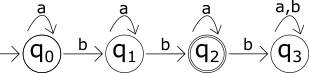
\includegraphics{img/automata4.png}
		\caption{Diagrama del autómata para $a^*ba^*ba^*$}
	\end{figure}
	
	\section*{Código fuente}
	
	\begin{lstlisting}[
		language=c,
		caption={Archivo cabecera},
		captionpos=b,
		breaklines=true,		
		]
\#include<stdio.h>

typedef struct Cadena\{
char * wn;
int longitud;
\}Cadena;

typedef struct Automata\{
int num\_estados;
int num\_simbolos;
int estado\_inicial;
int * estados\_finales;
int num\_finales;
int** transiciones;
\}Automata;

typedef Cadena * cadena;
typedef Automata * automata;

cadena crearCadena();
void pedirCadena(cadena);
void liberarCadena(cadena);


/*
num\_estados: numero de estados
num\_simbolos: numero de simbolos del alfabeto
estado\_inicial: estado inicial
estados\_finales: arreglo con los estados finales
transiciones: matriz de transiciones
*/
automata crearAutomata(int num\_estados, int num\_simbolos, int estado\_inicial,
int* estados\_finales, int num\_finales, int** transiciones);
int procesarCadena(automata, cadena);
void liberarAutomata(automata);
int crearAutomatas(automata automatas[4]);

void menuExpresiones(int, automata automatas[4]);
	\end{lstlisting}
	
	\cleardoublepage
	
	\begin{lstlisting}[
		language=c,
		caption={Implementación del archivo cabecera},
		captionpos=b,
		breaklines=true,		
		]
\#include<stdio.h>
\#include<stdlib.h>
\#include<unistd.h>
\#include``funciones.h''

cadena crearCadena()\{
cadena a;

a = (cadena)malloc(sizeof(Cadena));
if(a == NULL)\{
return NULL;
\}

a->wn = (char*)malloc(sizeof(char));
if(a->wn == NULL)\{
free(a);
return NULL;
\}

a->wn[0] = '\textbackslash{}0';
a->longitud = 0;

return a;
\}

void pedirCadena(cadena a)\{
scanf(``\%[\^{}\textbackslash{}n]s'',a->wn);
getchar();

int longitud = 0;
while(a->wn[longitud] != '\textbackslash{}0')\{
longitud++;
\}

a->longitud = longitud;
\}

void liberarCadena(cadena a)\{
if(a != NULL)\{
free(a->wn);
free(a);
\}
\}

automata crearAutomata(int num\_estados, int num\_simbolos, int estado\_inicial,
int* estados\_finales, int num\_finales, int** transiciones)\{

if(num\_estados<=0 || num\_simbolos<=0 || estado\_inicial<0 || num\_finales<0 || transiciones==NULL)\{
return NULL;
\}

automata a = (automata)malloc(sizeof(Automata));
if(a == NULL)\{
return NULL;
\}

a->num\_estados = num\_estados;
a->num\_simbolos = num\_simbolos;
a->estado\_inicial = estado\_inicial;
a->num\_finales = num\_finales;

a->estados\_finales = (int*)malloc(num\_finales * sizeof(int));
if(a->estados\_finales==NULL \&\& num\_finales>0)\{
free(a);
return NULL;
\}
for(int i=0; i<num\_finales; i++)\{
a->estados\_finales[i]=estados\_finales[i];
\}

a->transiciones = (int**)malloc(num\_estados * sizeof(int*));
if(a->transiciones == NULL)\{
free(a->estados\_finales);
free(a);
return NULL;
\}

for(int i = 0; i < num\_estados; i++) \{
a->transiciones[i] = (int*)malloc(num\_simbolos * sizeof(int));
if(a->transiciones[i] == NULL)\{
for(int j=0; j<i; j++)\{
free(a->transiciones[j]);
\}
free(a->transiciones);
free(a->estados\_finales);
free(a);
return NULL;
\}

for(int j=0; j<num\_simbolos; j++)\{
a->transiciones[i][j] = transiciones[i][j];
\}
\}

return a;
\}

int procesarCadena(automata a, cadena c)\{
if(a==NULL || c==NULL)\{
return 0;
\}

int estado\_actual = a->estado\_inicial;

printf(``\textbackslash{}n **** Transiciones del automata ****\textbackslash{}n\textbackslash{}n'');
for(int i=0; i<c->longitud; i++)\{
char ch = c->wn[i];
int simbolo = ch - 'a';
if(simbolo<0 || simbolo >= a->num\_simbolos)\{
printf(``Simbolo invalido [\%c]'', simbolo+'a');
return 0;
\}

int estado\_anterior = estado\_actual;
estado\_actual = a->transiciones[estado\_actual][simbolo];

printf(``Delta(q\%d, \%c)=q\%d\textbackslash{}n'', estado\_anterior, simbolo+'a', estado\_actual);
if(estado\_actual == -1)\{
return 0;
\}
\}

printf(``\textbackslash{}n\textbackslash{}n Estado final q\%d'', estado\_actual);

for(int i=0; i<a->num\_finales; i++)\{
if(a->estados\_finales[i] == estado\_actual)\{
return 1;
\}
\}

return 0;
\}

void liberarAutomata(automata a) \{
if (a == NULL) return;
for (int i = 0; i < a->num\_estados; i++) \{
free(a->transiciones[i]);
\}
free(a->transiciones);
free(a->estados\_finales);
free(a);
\}

int crearAutomatas(automata automatas[4]) \{
// Automata 1: a*ba*
int num\_estados1 = 3;
int num\_simbolos = 2;  // a, b
int inicial1 = 0;
int finales1[] = \{1\};
int num\_finales1 = 1;
int transiciones1[3][2] = \{
\{0, 1\},  // q0: a->q0, b->q1
\{1, 2\},  // q1: a->q1, b->q2 
\{2, 2\}   // q2: a->q2, b->q2
\};
int* transiciones\_ptr1[3] = \{transiciones1[0], transiciones1[1], transiciones1[2]\};

// Automata 2: a*bba*
int num\_estados2 = 4;
int inicial2 = 0;
int finales2[] = \{2\};
int num\_finales2 = 1;
int transiciones2[4][2] = \{
\{0, 1\},  // q0: a->q0, b->q1
\{3, 2\},  // q1: a->q3, b->q2
\{2, 3\},  // q2: a->q2, b->q3
\{3, 3\}   // q3: a->q3, b->q3
\};
int* transiciones\_ptr2[4] = \{transiciones2[0], transiciones2[1], transiciones2[2], transiciones2[3]\};

// Automata 3: a*b*
int num\_estados3 = 3;
int inicial3 = 0;
int finales3[] = \{0, 1\};  // q0 y q1 son finales
int num\_finales3 = 2;
int transiciones3[3][2] = \{
\{0, 1\},  // q0: a->q0, b->q1
\{2, 1\},  // q1: a->q2, b->q1
\{2, 2\}   // q2: a->q2, b->q2
\};
int* transiciones\_ptr3[3] = \{transiciones3[0], transiciones3[1], transiciones3[2]\};

// Automata 4: a*ba*ba*
int num\_estados4 = 4;
int inicial4 = 0;
int finales4[] = \{2\};
int num\_finales4 = 1;
int transiciones4[4][2] = \{
\{0, 1\},  // q0: a->q0, b->q1
\{1, 2\},  // q1: a->q1, b->q2
\{2, 3\},  // q2: a->q2, b->q3
\{3, 3\}   // q3: a->q3, b->q3
\};
int* transiciones\_ptr4[4] = \{transiciones4[0], transiciones4[1], transiciones4[2], transiciones4[3]\};

automatas[0] = crearAutomata(num\_estados1, num\_simbolos, inicial1,
finales1, num\_finales1, transiciones\_ptr1);
if (automatas[0] == NULL) return -1;

automatas[1] = crearAutomata(num\_estados2, num\_simbolos, inicial2,
finales2, num\_finales2, transiciones\_ptr2);
if (automatas[1] == NULL) \{
liberarAutomata(automatas[0]);
return -1;
\}

automatas[2] = crearAutomata(num\_estados3, num\_simbolos, inicial3,
finales3, num\_finales3, transiciones\_ptr3);
if (automatas[2] == NULL) \{
liberarAutomata(automatas[0]);
liberarAutomata(automatas[1]);
return -1;
\}

automatas[3] = crearAutomata(num\_estados4, num\_simbolos, inicial4,
finales4, num\_finales4, transiciones\_ptr4);
if (automatas[3] == NULL) \{
liberarAutomata(automatas[0]);
liberarAutomata(automatas[1]);
liberarAutomata(automatas[2]);
return -1;
\}

return 0;
\}

void menuExpresiones(int opc, automata automatas[4])\{
if (opc<1 || opc>4) return;

cadena cad = crearCadena();
if (cad == NULL) \{
printf(``Error al crear la cadena.\textbackslash{}n'');
return;
\}

printf(``Ingrese la cadena a evaluar (solo a y b, para cadena vacia solo presiona ENTER): '');
pedirCadena(cad);

if (procesarCadena(automatas[opc - 1], cad)) \{
printf(``\textbackslash{}tCADENA ACEPTADA\textbackslash{}n\textbackslash{}n'');
\} else \{
printf(``\textbackslash{}tCADENA RECHAZADA\textbackslash{}n\textbackslash{}n'');
\}

liberarCadena(cad);
\}

	\end{lstlisting}
	
	\cleardoublepage
	
	\begin{lstlisting}[
		language=c,
		caption={Implementación del archivo cabecera},
		captionpos=b,
		breaklines=true,		
		]
\#include<stdio.h>
\#include``funciones.h''

int main()\{
int opc;
printf(``\textbackslash{}n\textbackslash{}n\textbackslash{}t***** Practica 2 *****\textbackslash{}n'');

automata automatas[4];
if(crearAutomatas(automatas) != 0)\{
printf(``Error al crear los automatas, saliendo\textbackslash{}n'');
return 1;
\}

do\{
printf(``\textbackslash{}n Elija la expresion regular a revisar \textbackslash{}n\textbackslash{}n'');
printf(``1.- (a*)b(a*)\textbackslash{}n'');
printf(``2.- (a*)bb(a*)\textbackslash{}n'');
printf(``3.- a*b*\textbackslash{}n'');
printf(``4.- (a*)b(a*)b(a*)\textbackslash{}n'');
printf(``5.- Salir\textbackslash{}n\textbackslash{}n'');

scanf(``\%d'', \&opc);
getchar();

if(opc>=1 \&\& opc<=4)\{
menuExpresiones(opc, automatas);
\}else if(opc != 5)\{
printf(``Opcion invalida, intente de nuevo\textbackslash{}n'');
\}
\}while(opc != 5);

for(int i=0; i<4; i++)\{
liberarAutomata(automatas[i]);
\}


return 0;
\}
	\end{lstlisting}
	
	\newpage
	
	\section*{Pruebas de código}

	\subsection*{Autómata 1}
	El primer paso es tener la lista de cadenas que pertenecen al lenguaje. $L=\{b,ab,ba,aba,aaba,aabaa\}$, ahora se prueba una a una las cadenas en el programa.

	\begin{figure}[H]
    \centering
    \begin{minipage}{0.48\textwidth}
        \centering
        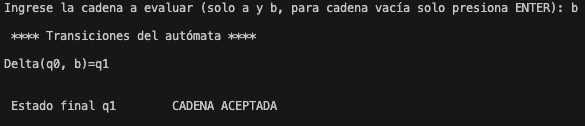
\includegraphics[width=\textwidth]{img/a11.png}
        \caption*{Prueba con 'b'}
    \end{minipage}
    \hfill
    \begin{minipage}{0.48\textwidth}
        \centering
        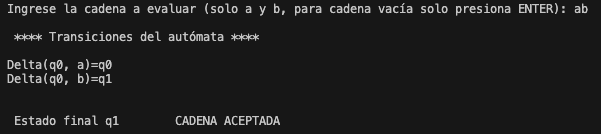
\includegraphics[width=\textwidth]{img/a12.png}
        \caption*{Prueba con 'ab'}
    \end{minipage}
	\begin{minipage}{0.48\textwidth}
        \centering
        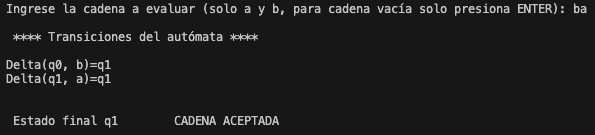
\includegraphics[width=\textwidth]{img/a13.png}
        \caption*{Prueba con 'ba'}
    \end{minipage}
    \hfill
    \begin{minipage}{0.48\textwidth}
        \centering
        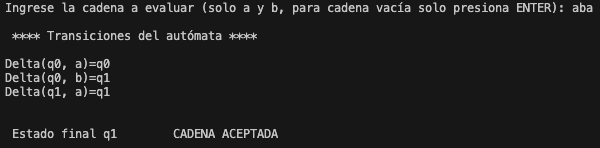
\includegraphics[width=\textwidth]{img/a14.png}
        \caption*{Prueba con 'aba'}
    \end{minipage}
	\begin{minipage}{0.48\textwidth}
        \centering
        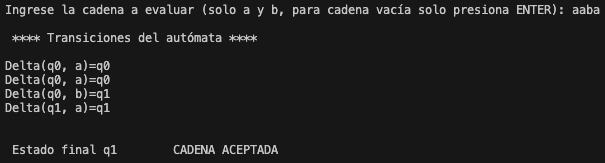
\includegraphics[width=\textwidth]{img/a15.png}
        \caption*{Prueba con 'aaba'}
    \end{minipage}
    \hfill
    \begin{minipage}{0.48\textwidth}
        \centering
        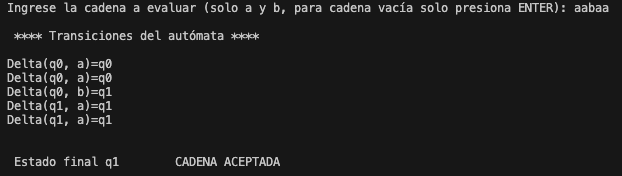
\includegraphics[width=\textwidth]{img/a16.png}
        \caption*{Prueba con 'aabaa'}
    \end{minipage}
\end{figure}

	Ahora probaremos con cadenas que no pertenecen al lenguaje como $L=\{bab,baab,aabaab,bb,bba\}$

\begin{figure}[H]
    \centering
    \begin{minipage}{0.48\textwidth}
        \centering
        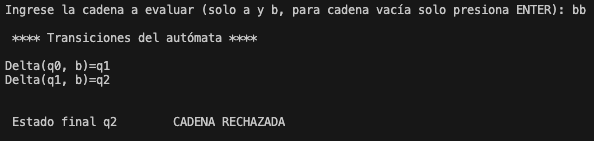
\includegraphics[width=\textwidth]{img/a17.png}
        \caption*{Prueba con 'bab'}
    \end{minipage}
    \hfill
    \begin{minipage}{0.48\textwidth}
        \centering
        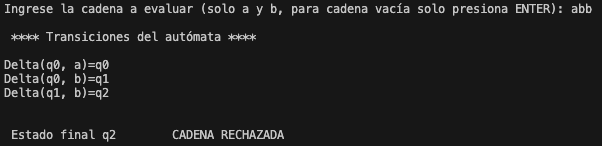
\includegraphics[width=\textwidth]{img/a18.png}
        \caption*{Prueba con 'baab'}
    \end{minipage}
	\begin{minipage}{0.48\textwidth}
        \centering
        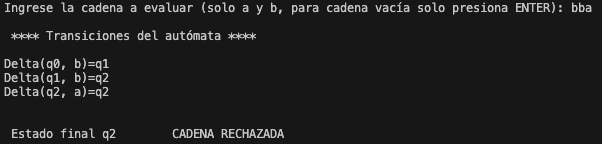
\includegraphics[width=\textwidth]{img/a19.png}
        \caption*{Prueba con 'aabaab'}
    \end{minipage}
    \hfill
    \begin{minipage}{0.48\textwidth}
        \centering
        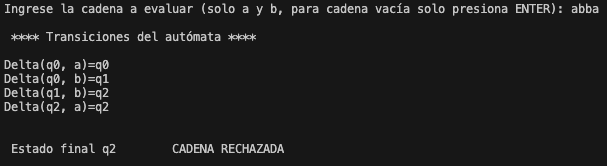
\includegraphics[width=\textwidth]{img/a110.png}
        \caption*{Prueba con 'bb'}
    \end{minipage}
	\begin{minipage}{0.48\textwidth}
        \centering
        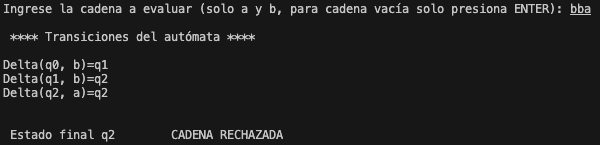
\includegraphics[width=\textwidth]{img/a111.png}
        \caption*{Prueba con 'bba'}
    \end{minipage}
    \hfill
\end{figure}

	Por último se prueba la cadena vacía y símbolos fuera del alfabeto
\begin{figure}[H]
    \centering
    \begin{minipage}{0.48\textwidth}
        \centering
        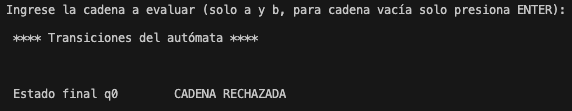
\includegraphics[width=\textwidth]{img/a112.png}
        \caption*{Prueba con cadena vacía}
    \end{minipage}
    \hfill
    \begin{minipage}{0.48\textwidth}
        \centering
        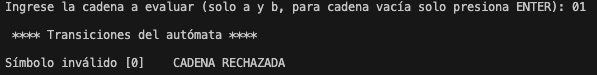
\includegraphics[width=\textwidth]{img/a113.png}
        \caption*{Prueba con símbolos fuera del alfabeto}
    \end{minipage}
\end{figure}

	\subsection*{Autómata 2}
	El primer paso es tener la lista de cadenas que pertenecen al lenguaje. $L=\{bb,abb,bba,abba,aaabb,bbaaaa\}$, ahora se prueba una a una las cadenas en el programa.

	\begin{figure}[H]
    \centering
    \begin{minipage}{0.48\textwidth}
        \centering
        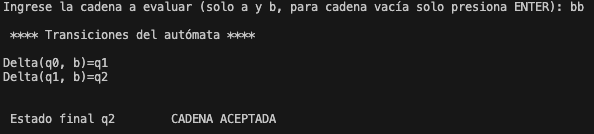
\includegraphics[width=\textwidth]{img/a21.png}
        \caption*{Prueba con 'bb'}
    \end{minipage}
    \hfill
    \begin{minipage}{0.48\textwidth}
        \centering
        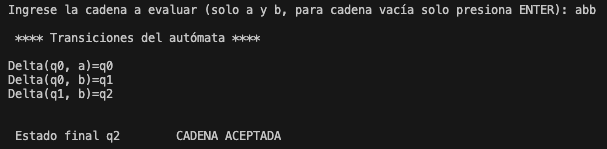
\includegraphics[width=\textwidth]{img/a22.png}
        \caption*{Prueba con 'abb'}
    \end{minipage}
	\begin{minipage}{0.48\textwidth}
        \centering
        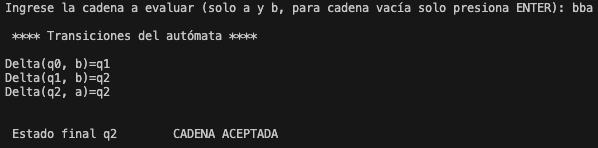
\includegraphics[width=\textwidth]{img/a23.png}
        \caption*{Prueba con 'bba'}
    \end{minipage}
    \hfill
    \begin{minipage}{0.48\textwidth}
        \centering
        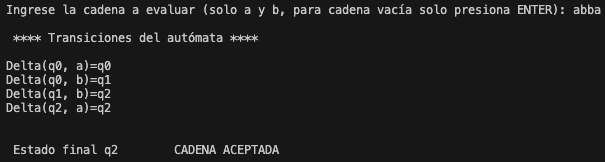
\includegraphics[width=\textwidth]{img/a24.png}
        \caption*{Prueba con 'abba'}
    \end{minipage}
	\begin{minipage}{0.48\textwidth}
        \centering
        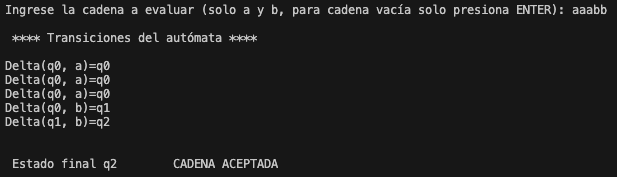
\includegraphics[width=\textwidth]{img/a25.png}
        \caption*{Prueba con 'aaabb'}
    \end{minipage}
    \hfill
    \begin{minipage}{0.48\textwidth}
        \centering
        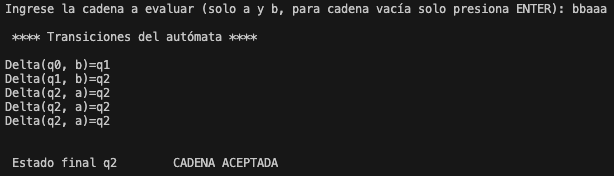
\includegraphics[width=\textwidth]{img/a26.png}
        \caption*{Prueba con 'bbaaaa'}
    \end{minipage}
\end{figure}

	Ahora probaremos con cadenas que no pertenecen al lenguaje como $L=\{ba,aba,bbb,bbba,abbb\}$

\begin{figure}[H]
    \centering
    \begin{minipage}{0.48\textwidth}
        \centering
        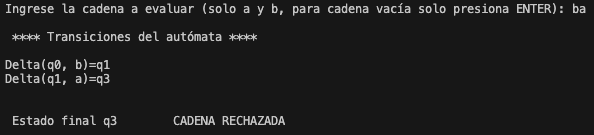
\includegraphics[width=\textwidth]{img/a27.png}
        \caption*{Prueba con 'ba'}
    \end{minipage}
    \hfill
    \begin{minipage}{0.48\textwidth}
        \centering
        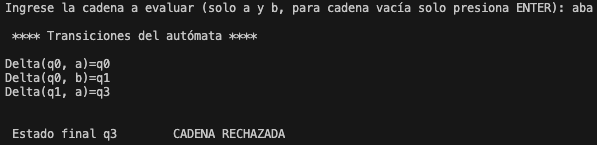
\includegraphics[width=\textwidth]{img/a28.png}
        \caption*{Prueba con 'aba'}
    \end{minipage}
	\begin{minipage}{0.48\textwidth}
        \centering
        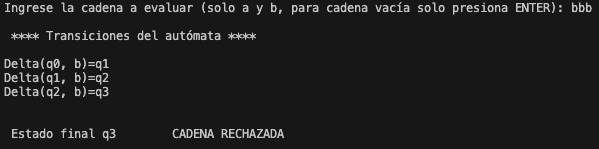
\includegraphics[width=\textwidth]{img/a29.png}
        \caption*{Prueba con 'bbb'}
    \end{minipage}
    \hfill
    \begin{minipage}{0.48\textwidth}
        \centering
        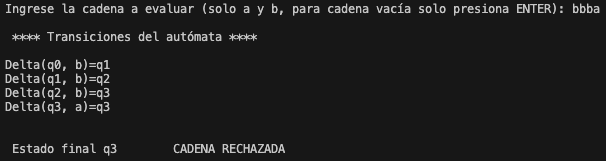
\includegraphics[width=\textwidth]{img/a210.png}
        \caption*{Prueba con 'bbba'}
    \end{minipage}
	\begin{minipage}{0.48\textwidth}
        \centering
        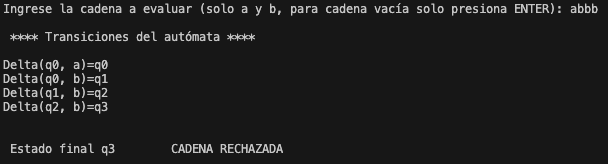
\includegraphics[width=\textwidth]{img/a211.png}
        \caption*{Prueba con 'abbb'}
    \end{minipage}
    \hfill
\end{figure}

	Por último se prueba la cadena vacía y símbolos fuera del alfabeto
\begin{figure}[H]
    \centering
    \begin{minipage}{0.48\textwidth}
        \centering
        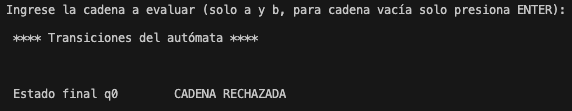
\includegraphics[width=\textwidth]{img/a112.png}
        \caption*{Prueba con cadena vacía}
    \end{minipage}
    \hfill
    \begin{minipage}{0.48\textwidth}
        \centering
        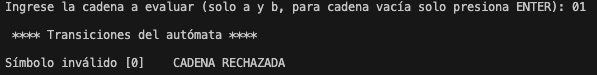
\includegraphics[width=\textwidth]{img/a113.png}
        \caption*{Prueba con símbolos fuera del alfabeto}
    \end{minipage}
\end{figure}

	\subsection*{Autómata 3}
	El primer paso es tener la lista de cadenas que pertenecen al lenguaje. $L=\{\lambda,a,b,aabb,aa,bb\}$, ahora se prueba una a una las cadenas en el programa.

	\begin{figure}[H]
    \centering
    \begin{minipage}{0.48\textwidth}
        \centering
        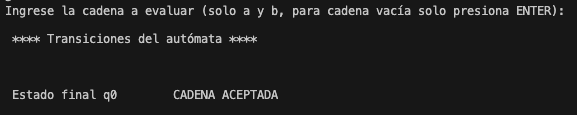
\includegraphics[width=\textwidth]{img/a31.png}
        \caption*{Prueba con cadena vacía}
    \end{minipage}
    \hfill
    \begin{minipage}{0.48\textwidth}
        \centering
        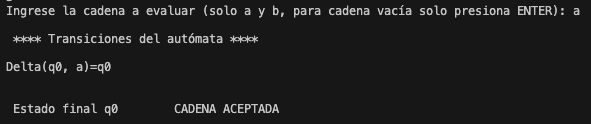
\includegraphics[width=\textwidth]{img/a32.png}
        \caption*{Prueba con 'a'}
    \end{minipage}
	\begin{minipage}{0.48\textwidth}
        \centering
        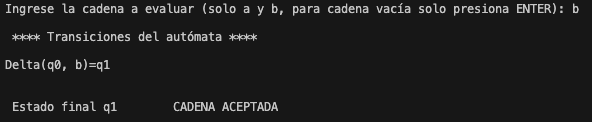
\includegraphics[width=\textwidth]{img/a33.png}
        \caption*{Prueba con 'b'}
    \end{minipage}
    \hfill
    \begin{minipage}{0.48\textwidth}
        \centering
        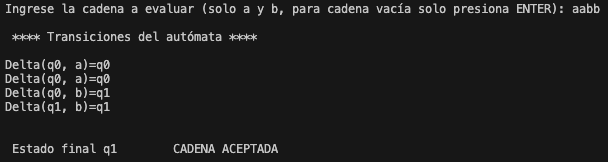
\includegraphics[width=\textwidth]{img/a34.png}
        \caption*{Prueba con 'aabb'}
    \end{minipage}
	\begin{minipage}{0.48\textwidth}
        \centering
        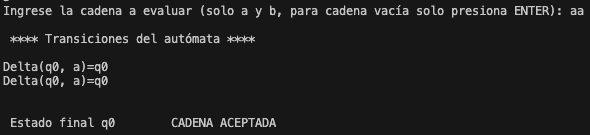
\includegraphics[width=\textwidth]{img/a35.png}
        \caption*{Prueba con 'aa'}
    \end{minipage}
    \hfill
    \begin{minipage}{0.48\textwidth}
        \centering
        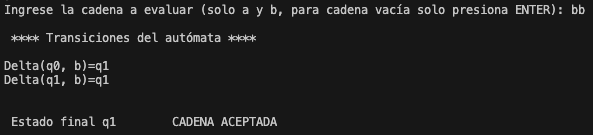
\includegraphics[width=\textwidth]{img/a36.png}
        \caption*{Prueba con 'bb'}
    \end{minipage}
\end{figure}

	Ahora probaremos con cadenas que no pertenecen al lenguaje como $L=\{ba,aba,bab,bbba,abbba\}$

\begin{figure}[H]
    \centering
    \begin{minipage}{0.48\textwidth}
        \centering
        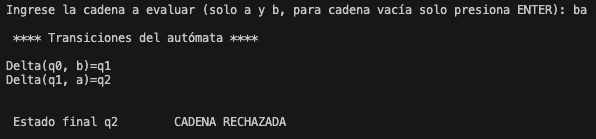
\includegraphics[width=\textwidth]{img/a37.png}
        \caption*{Prueba con 'ba'}
    \end{minipage}
    \hfill
    \begin{minipage}{0.48\textwidth}
        \centering
        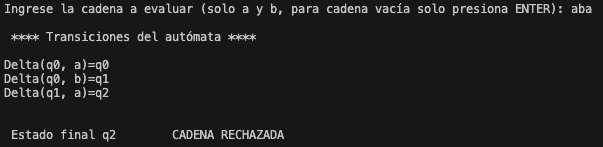
\includegraphics[width=\textwidth]{img/a38.png}
        \caption*{Prueba con 'aba'}
    \end{minipage}
	\begin{minipage}{0.48\textwidth}
        \centering
        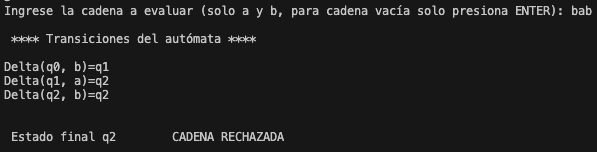
\includegraphics[width=\textwidth]{img/a39.png}
        \caption*{Prueba con 'bab'}
    \end{minipage}
    \hfill
    \begin{minipage}{0.48\textwidth}
        \centering
        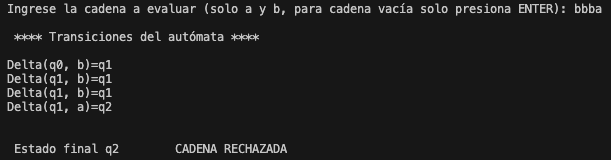
\includegraphics[width=\textwidth]{img/a310.png}
        \caption*{Prueba con 'bbba'}
    \end{minipage}
	\begin{minipage}{0.48\textwidth}
        \centering
        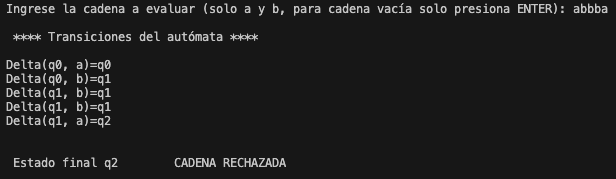
\includegraphics[width=\textwidth]{img/a311.png}
        \caption*{Prueba con 'abbba'}
    \end{minipage}
    \hfill
\end{figure}

	Por último se prueba la cadena vacía y símbolos fuera del alfabeto
\begin{figure}[H]
    \centering
    \begin{minipage}{0.48\textwidth}
        \centering
        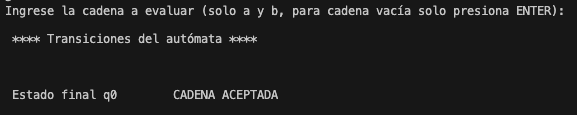
\includegraphics[width=\textwidth]{img/a31.png}
        \caption*{Prueba con cadena vacía}
    \end{minipage}
    \hfill
    \begin{minipage}{0.48\textwidth}
        \centering
        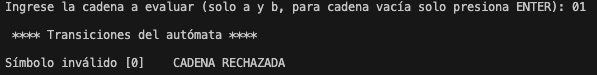
\includegraphics[width=\textwidth]{img/a113.png}
        \caption*{Prueba con símbolos fuera del alfabeto}
    \end{minipage}
\end{figure}

	\subsection*{Autómata 4}
	El primer paso es tener la lista de cadenas que pertenecen al lenguaje. $L=\{bb,abb,bab,bba,aabaabaa\}$, ahora se prueba una a una las cadenas en el programa.

	\begin{figure}[H]
    \centering
    \begin{minipage}{0.48\textwidth}
        \centering
        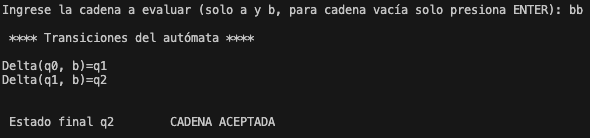
\includegraphics[width=\textwidth]{img/a41.png}
        \caption*{Prueba con 'bb'}
    \end{minipage}
    \hfill
    \begin{minipage}{0.48\textwidth}
        \centering
        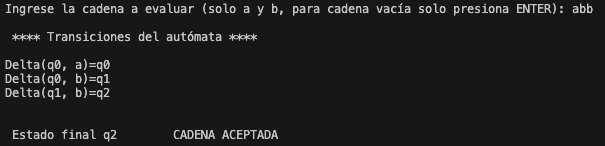
\includegraphics[width=\textwidth]{img/a42.png}
        \caption*{Prueba con 'abb'}
    \end{minipage}
	\begin{minipage}{0.48\textwidth}
        \centering
        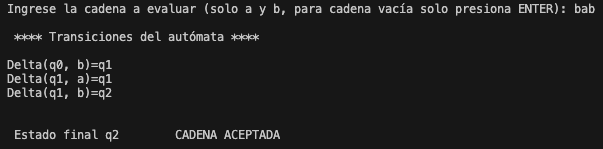
\includegraphics[width=\textwidth]{img/a43.png}
        \caption*{Prueba con 'bab'}
    \end{minipage}
    \hfill
    \begin{minipage}{0.48\textwidth}
        \centering
        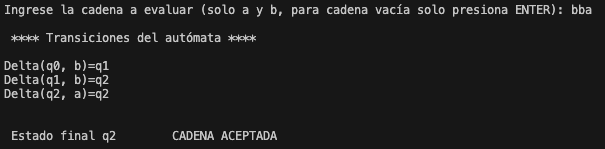
\includegraphics[width=\textwidth]{img/a44.png}
        \caption*{Prueba con 'bba'}
    \end{minipage}
	\begin{minipage}{0.48\textwidth}
        \centering
        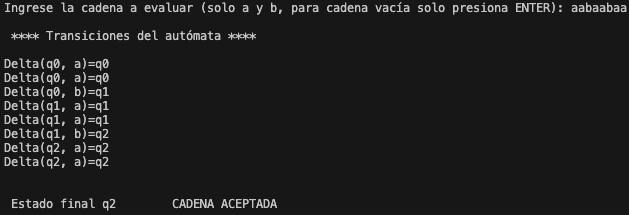
\includegraphics[width=\textwidth]{img/a45.png}
        \caption*{Prueba con 'aabaabaa'}
    \end{minipage}
\end{figure}

	Ahora probaremos con cadenas que no pertenecen al lenguaje como $L=\{ba,aba,babb,bbba,abbba\}$

\begin{figure}[H]
    \centering
    \begin{minipage}{0.48\textwidth}
        \centering
        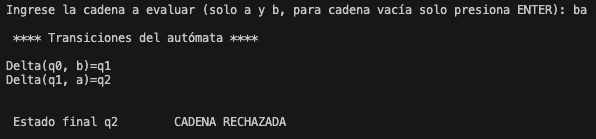
\includegraphics[width=\textwidth]{img/a37.png}
        \caption*{Prueba con 'ba'}
    \end{minipage}
    \hfill
    \begin{minipage}{0.48\textwidth}
        \centering
        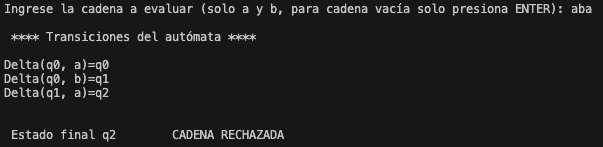
\includegraphics[width=\textwidth]{img/a38.png}
        \caption*{Prueba con 'aba'}
    \end{minipage}
	\begin{minipage}{0.48\textwidth}
        \centering
        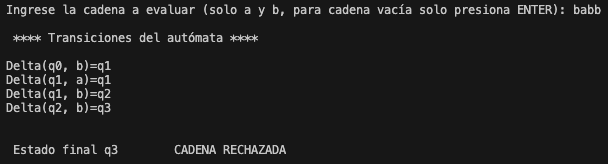
\includegraphics[width=\textwidth]{img/a46.png}
        \caption*{Prueba con 'babb'}
    \end{minipage}
    \hfill
    \begin{minipage}{0.48\textwidth}
        \centering
        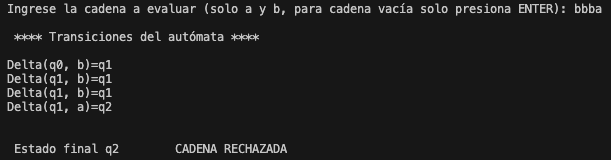
\includegraphics[width=\textwidth]{img/a310.png}
        \caption*{Prueba con 'bbba'}
    \end{minipage}
	\begin{minipage}{0.48\textwidth}
        \centering
        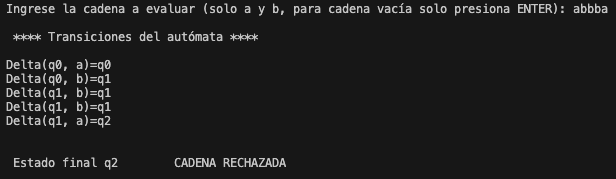
\includegraphics[width=\textwidth]{img/a311.png}
        \caption*{Prueba con 'abbba'}
    \end{minipage}
    \hfill
\end{figure}

	Por último se prueba la cadena vacía y símbolos fuera del alfabeto
\begin{figure}[H]
    \centering
    \begin{minipage}{0.48\textwidth}
        \centering
        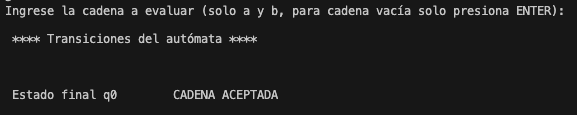
\includegraphics[width=\textwidth]{img/a31.png}
        \caption*{Prueba con cadena vacía}
    \end{minipage}
    \hfill
    \begin{minipage}{0.48\textwidth}
        \centering
        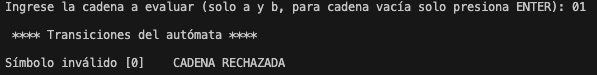
\includegraphics[width=\textwidth]{img/a113.png}
        \caption*{Prueba con símbolos fuera del alfabeto}
    \end{minipage}
\end{figure}
	
	\section*{Relación entre Especificación Formal e Implementación}
	La implementación en C refleja fielmente la teoría de autómatas mediante los siguientes mapeos de componentes:
	
	\begin{itemize}
		\item \textbf{Estados ($Q$):} Representados por el campo \texttt{num\_estados} y gestionados mediante índices enteros en la matriz de transiciones.
		\item \textbf{Alfabeto ($\Sigma$):} Aunque el programa acepta caracteres, estos se mapean a índices enteros mediante la operación \texttt{ch - 'a'}, restringiendo el alfabeto a $\{a, b\}$.
		\item \textbf{Función de Transición ($\delta$):} Se implementa como una matriz bidimensional (\texttt{int** transiciones}), donde \texttt{transiciones[estado\_actual][simbolo]} devuelve el siguiente estado.
		\item \textbf{Estado Inicial ($q_0$):} Almacenado explícitamente en el campo \texttt{estado\_inicial} de la estructura \texttt{Automata}.
		\item \textbf{Estados Finales ($F$):} Un arreglo dinámico (\texttt{estados\_finales}) que el programa recorre al finalizar el procesamiento de la cadena para determinar la aceptación.
	\end{itemize}
	
	El corazón del procesamiento reside en la función \texttt{procesarCadena}, que emula la función de transición $\delta$, iterando sobre la cadena y actualizando el estado actual hasta consumir toda la entrada o alcanzar un estado de error (-1).
	
\end{document}